\documentclass[letterpaper,12pt,fleqn]{article}
\usepackage{matharticle}
\usepackage{mathtools}
\pagestyle{plain}
\begin{document}

\begin{center}
\Large Math-08 Homework \#8 Solutions
\end{center}

\vspace{0.5in}

\underline{Reading}

\begin{itemize}
\item Text book section 1.2,1.6,1.7
\end{itemize}

\underline{Problems}

\begin{enumerate}

\item You are a product manager at an electronics firm in charge of a proposed
  new line of 25-inch monitors (i.e., the length of the diagonal across the
  screen is 25 inches):

  \bigskip

  \begin{figure}[h]
    \setlength{\leftskip}{1in}
    \begin{tikzpicture}
      \draw (0,0) rectangle (5,3);
      \draw [dashed] (0,0) -- (5,3);
      \node at (2.5,2.0) {25''};
      \node [above] at (2.5,0) {$\ell$};
      \node [right] at (0,1.5) {$w$};
    \end{tikzpicture}
  \end{figure}

  You realize that the most appealing ratio for the dimensions of the screen
  would follow the golden ratio:
  \[\frac{\ell}{w}=\frac{1+\sqrt{5}}{2}\approx1.6=\frac{8}{5}\]

  \begin{enumerate}
  \item Using the estimate of $8/5$, determine the dimensions ($\ell\times w$)
    for the new monitor. Round each dimension to two decimal places.

    \bigskip

    Note that we have a right triangle with a hypotenuse of 25 inches. Thus:
    \[w^2+\ell^2=25^2\]
    Let's pick $w$ to be our key unknown. So we need to define $l$ in terms of
    $w$:
    \[\frac{\ell}{w}=\frac{8}{5}\]
    \[5\ell=8w\]
    \[\ell=\frac{8}{5}w\]
    Now, plug in and solve:
    \[w^2+\left(\frac{8}{5}w\right)^2=25^2\]
    \[w^2+\frac{64}{25}w^2=625\]
    \[\frac{89}{25}w^2=625\]
    \[w^2=\frac{625(25)}{89}\]
    \[w=\sqrt{\frac{625(25)}{89}}\]
    \[w=13.25\]
    \[\ell=\frac{8}{5}13.25=21.20\]
    Dimensions$=21.20$ in $\times13.25$ in

    \bigskip

  \item There needs to be an equal amount of casing around the edges of the
    screen and the packaging department would like the monitor to have a total
    area of 400 square inches.

    \begin{figure}[h]
      \setlength{\leftskip}{1in}
      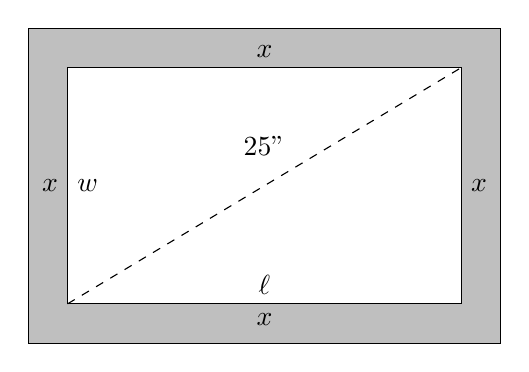
\begin{tikzpicture}
        \draw [fill=lightgray] (-0.5,-0.5) rectangle (5.5,3.5);
        \draw [fill=white] (0,0) rectangle (5,3);
        \draw [dashed] (0,0) -- (5,3);
        \node at (2.5,2.0) {25''};
        \node [above] at (2.5,0) {$\ell$};
        \node [right] at (0,1.5) {$w$};
        \node [above] at (2.5,3) {$x$};
        \node [below] at (2.5,0) {$x$};
        \node [left] at (0,1.5) {$x$};
        \node [right] at (5,1.5) {$x$};
      \end{tikzpicture}
    \end{figure}

    Determine the width of the casing ($x$) around the screen. Round your
    answer to two decimal places.

    \[(2x+21.20)(2x+13.25)=400\]
    \[4x^2+68.9x+280.9=400\]
    \[4x^2+68.9x-119.1=0\]
    \[x=\frac{-68.9\pm\sqrt{68.9^2-4(4)(-119.1)}}{2(4)}=1.58\]
    The border should be $1.58$ in.
  \end{enumerate}

  \bigskip

\item A man stands atop a 256 foot cliff with a ball.
  \begin{enumerate}
  \item How long does it take for the ball to hit the ground if he simply
    releases the ball?
    \[0=256-16t^2\]
    \[16t^2=256\]
    \[t^2=16\]
    \[\abs{t}=4\]
    \[t=\pm4\]
    The ball hits the ground in 4 seconds.

    \bigskip

  \item How long does it take for the ball to hit the ground if he throws the
    ball up with a velocity of 16 ft/s? (Hint: keep the negative solution
    around for later).
    \[0=256+16t-16t^2\]
    \[0=16+t-t^2\]
    \[t^2-t-16=0\]
    \[t=\frac{1\pm\sqrt{(-1)^2-4(-1)(16)}}{2(1)}=4.5, -3.5\]
    The ball hits the ground in 4.5 seconds.

  \item How long does it take for the ball to hit the ground if he throws the
    ball down with a velocity of 16 ft/s? (Hint: no additional calculations
    are needed).

    \bigskip

    The ball hits the ground in 3.5 seconds (the negative result from the
    previous part).

  \item Assume that a lady is standing on the ground below the cliff and throws
    a ball up so that it passed the man on the cliff at a velocity of 16 ft/s.
    How long would it be before the ball hits the ground? (Hint: you already
    have all the information that you need).

    \bigskip

    The ball hits the ground in $4.5+3.5=8 seconds$, which is the sum of the
    two paths in the previous two parts.
\end{enumerate}

  \bigskip

\item For each of the following inequalities, graph the solution set and
  state the solution set in interval notation.
  \begin{enumerate}
  \item $2\abs{5-3x}+7<21$

    We want to get the inequality into standard form first:
    \[2\abs{5-3x}<14\]
    \[\abs{5-3x}<7\]
    Now that it is in standard form, and is a ``less than'' problem, we can
    make the corresponding compound inequality and solve simultaneously for
    $x$:
    \[-7<5-3x<7\]
    \[-12<-3x<2\]
    \[4>x>-\frac{2}{3}\]
    \[-\frac{2}{3}<x<4\]
    Note that in the last steps we multiplied by a negative number, so we
    needed to flip the inequality signs. The resulting graph is as follows:

    \bigskip

    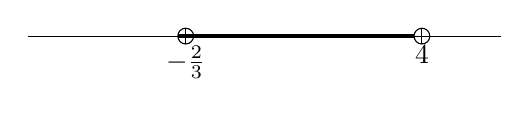
\begin{tikzpicture}
      \draw (-3,0) -- (3,0);
      \draw (-1,0.1) -- (-1,-0.1);
      \draw (2,0.1) -- (2,-0.1);
      \draw (-1,0) circle [radius=0.1];
      \draw (2,0) circle [radius=0.1];
      \node [below] at (-1,0) {$-\frac{2}{3}$};
      \node [below] at (2,0) {$4$};
      \draw [ultra thick] (-1.1,0) -- (1.9,0);
    \end{tikzpicture}

    \bigskip

    And the corresponding interval notation is: $\left(-\frac{2}{3},4\right)$
    
  \item $2\abs{5-3x}+7\ge21$

    Instead of the inside, we want the outside. Also, since we are allowing
    equality, we include the endpoints.  The resulting graph is as follows:

    \bigskip

    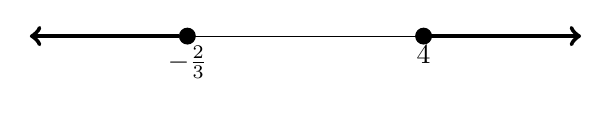
\begin{tikzpicture}
      \draw (-3,0) -- (3,0);
      \draw (-1,0.1) -- (-1,-0.1);
      \draw (2,0.1) -- (2,-0.1);
      \draw [fill=black] (-1,0) circle [radius=0.1];
      \draw [fill=black] (2,0) circle [radius=0.1];
      \node [below] at (-1,0) {$-\frac{2}{3}$};
      \node [below] at (2,0) {$4$};
      \draw [<-,ultra thick] (-3,0) -- (-1.1,0);
      \draw [->,ultra thick] (2.1,0) -- (4,0);
    \end{tikzpicture}
    
    \bigskip

    And the resulting interval notation is:
    $\left(-\infty,-\frac{2}{3}\right]\cup\left[4,\infty\right)$

    \bigskip
  \end{enumerate}

\item Solve for $x$, stating the solution in interval notation.
  \[\frac{x+1}{x-2}<\frac{x-3}{x+4}\]
  Remember, we cannot cross multiply here because we don't yet know if we might
  be multiplying by a negative number. Instead, we bring everything to one
  side and combine using the fraction rules from 0.2:
  \[\frac{x+1}{x-2}-\frac{x-3}{x+4}<0\]
  \[\frac{(x+1)(x+4)-(x-2)(x-3)}{(x-2)(x+4)}<0\]
  \[\frac{(x^2+5x+4)-(x^2-5x+6)}{(x-2)(x+4)}<0\]
  \[\frac{(10x-2)}{(x-2)(x+4)}<0\]
  As an optional step, let's factor out the 10 from the factor in the
  numerator. Note that it is a positive constant, so it will not affect the
  sign. In fact, if we multipl both sides by $\frac{1}{10}$, it just goes
  away:
  \[\frac{10(x-\frac{1}{5})}{(x-2)(x+4)}<0\]
  \[\frac{(x-\frac{1}{5})}{(x-2)(x+4)}<0\]
  Remember, if it had been a $-10$ then we would need to flip the inequality
  sign. We are now ready to build a sign table. Remember to include both the
  zeros and the poles, since we can change sign across either:

  \begin{tabular}{c|ccc|c}
    test & $(x-\frac{1}{5})$ & $(x-2)$ & $(x+4)$ & sign \\
    \hline
    $-5$ & $-$ & $-$ & $-$ & $-$ \\
    $0$ & $-$ & $-$ & $+$ & $+$ \\
    $1$ & $+$ & $-$ & $+$ & $-$ \\
    $3$ & $+$ & $+$ & $+$ & $+$ \\
  \end{tabular}

  \bigskip

  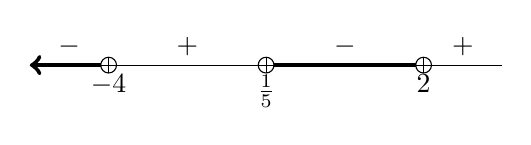
\begin{tikzpicture}
    \draw (-3,0) -- (3,0);
    \draw (-2,0.1) -- (-2,-0.1);
    \draw (0,0.1) -- (0,-0.1);
    \draw (2,0.1) -- (2,-0.1);
    \draw (-2,0) circle [radius=0.1];
    \draw (0,0) circle [radius=0.1];
    \draw (2,0) circle [radius=0.1];
    \node [below] at (-2,0) {$-4$};
    \node [below] at (0,0) {$\frac{1}{5}$};
    \node [below] at (2,0) {$2$};
    \node [above] at (-2.5,0) {$-$};
    \node [above] at (-1,0) {$+$};
    \node [above] at (1,0) {$-$};
    \node [above] at (2.5,0) {$+$};
    \draw [<-,ultra thick] (-3,0) -- (-2.1,0);
    \draw [ultra thick] (0.1,0) -- (1.9,0);
  \end{tikzpicture}
    
  \bigskip

  Since the inequality is ``less than'' we want all of the negative intervals.
  Note that since equality is not allowed, all endpoints are not included:
  \[(-\infty,-4)\cup\left(\frac{1}{5},2\right)\]

\item Determine the domain for each of the following expressions, stating each
  in interval notation.
  \begin{enumerate}
  \item \[\sqrt{\frac{x^2-3x-10}{x^2-9x+20}}\]

    This is a square (even) root, so negative radicands are not allowed. We
    turn this into an inequality:
    \[\frac{x^2-3x-10}{x^2-9x+20}\ge0\]
    We need the numerator and denominator in factored form so that we can
    build a sign table:
    \[\frac{(x-5)(x+2)}{(x-5)(x-4)}\ge0\]
    Now we note that the $(x-5)$ factor cancels; however, we need to remember
    that $5$ is not in the domain - we will need a hole there:
    \[\frac{x+2}{x-4}\ge0\]
    We are now ready to build the sign table:

    \begin{tabular}{c|cc|c}
      test & $(x+2)$ & $(x-4)$ & sign \\
      \hline
      -3 & $-$ & $-$ & $+$ \\
      0 & $+$ & $-$ & $-$ \\
      5 & $+$ & $+$ & $+$ \\
    \end{tabular}
    
    \bigskip

    And don't forget the hole at $5$:

    \bigskip

    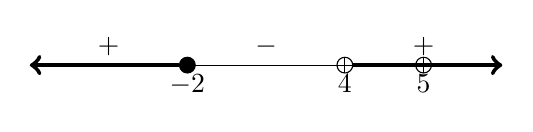
\begin{tikzpicture}
      \draw (-3,0) -- (3,0);
      \draw (-1,0.1) -- (-1,-0.1);
      \draw (1,0.1) -- (1,-0.1);
      \draw (2,0.1) -- (2,-0.1);
      \draw [fill=black] (-1,0) circle [radius=0.1];
      \draw (1,0) circle [radius=0.1];
      \draw (2,0) circle [radius=0.1];
      \node [below] at (-1,0) {$-2$};
      \node [below] at (1,0) {$4$};
      \node [below] at (2,0) {$5$};
      \node [above] at (-2,0) {$+$};
      \node [above] at (0,0) {$-$};
      \node [above] at (2,0) {$+$};
      \draw [<-,ultra thick] (-3,0) -- (-1.1,0);
      \draw [ultra thick] (1.1,0) -- (1.9,0);
      \draw [->,ultra thick] (1.9,0) -- (3,0);
    \end{tikzpicture}
    
    \bigskip

    Note that equality is allowed here, so zeros (-2) are included, but poles
    (4)are still excluded. So the domain is:
    \[(-\infty,-2]\cup(4,5)\cup(5,\infty)\]

  \item \[\sqrt[3]{\frac{x^2-3x-10}{x^2-9x+20}}\]
      
  This is an \emph{odd} root, so there is no need to worry about a negative
  radicand. We still need to be cautious of a zero denominator, through, so
  based on the answer to the previous part, we just need to leave holes at
  $x=4,5$:
  \[(-\infty,4)\cup(4,5)\cup(5,\infty)\]
  
  \end{enumerate}
\end{enumerate}
  
\end{document}
